\documentclass{article}
\usepackage{graphicx}
\usepackage{amsmath}
\usepackage{soul}
\usepackage{color}
\usepackage{float}
\usepackage{stfloats}
\usepackage[a4paper, margin=1in]{geometry}
\usepackage{xr}
\externaldocument{sensors_metal_main}

\renewcommand{\thesection}{S\arabic{section}}
\setcounter{section}{0}
\renewcommand{\thesubsection}{S\arabic{section}.\arabic{subsection}}
\setcounter{subsection}{0}
\renewcommand{\thefigure}{S.\arabic{figure}}
\setcounter{figure}{0}
\renewcommand{\thetable}{S.\arabic{table}}
\setcounter{table}{0}

\begin{document}
\title{Supplementary Material for\\ “Evaluation of Metallic Interference in Electromagnetic Tracker for Handheld Robotics”}
\author{Poonnapa Chaichudchaval, Robert A. MacLachlan, \\and Cameron N. Riviere}
\maketitle

\section{Metal sample details}
\label{supplement: sample_weight}
\begin{table}[!htbp]
\caption{Weight of Samples}
\label{mat_size}
\setlength{\tabcolsep}{3pt}
\centering
\begin{tabular}{|l|c|c|c|c|}
\hline
\parbox{60pt}{\centering {Metal Type}} & 
\parbox{45pt}{\centering {Rod (g)}} & 
\parbox{45pt}{\centering {Tube (g)}} & 
\parbox{45pt}{\centering {Sheet (g)}}\\
\hline
LC steel& $34.51$& $39.29$&$900$\\
416 SS& $34.55$& $38.63$&$ $\\
304 SS& $36.28$& $39.35$&$840$\\
6061 Al& $12.36$& $13.37$&$300$\\
Ti& $19.22$& $22.67$&$ $ \\
Cu& $39.69$& $45.05$&$1000$ \\
\hline
\end{tabular}
\end{table}

The weights of all metal samples are shown in Table \ref{mat_size}. The rod and tube samples are the same length and were fabricated with the same nominal metal (within the constraints of stock metal shapes), so the masses are similar for each metal type. The sheets are much larger, with correspondingly higher mass.

\section{Tracker configuration}
\label{supplement:tracker_configuration}
\begin{figure}[H]
\centerline{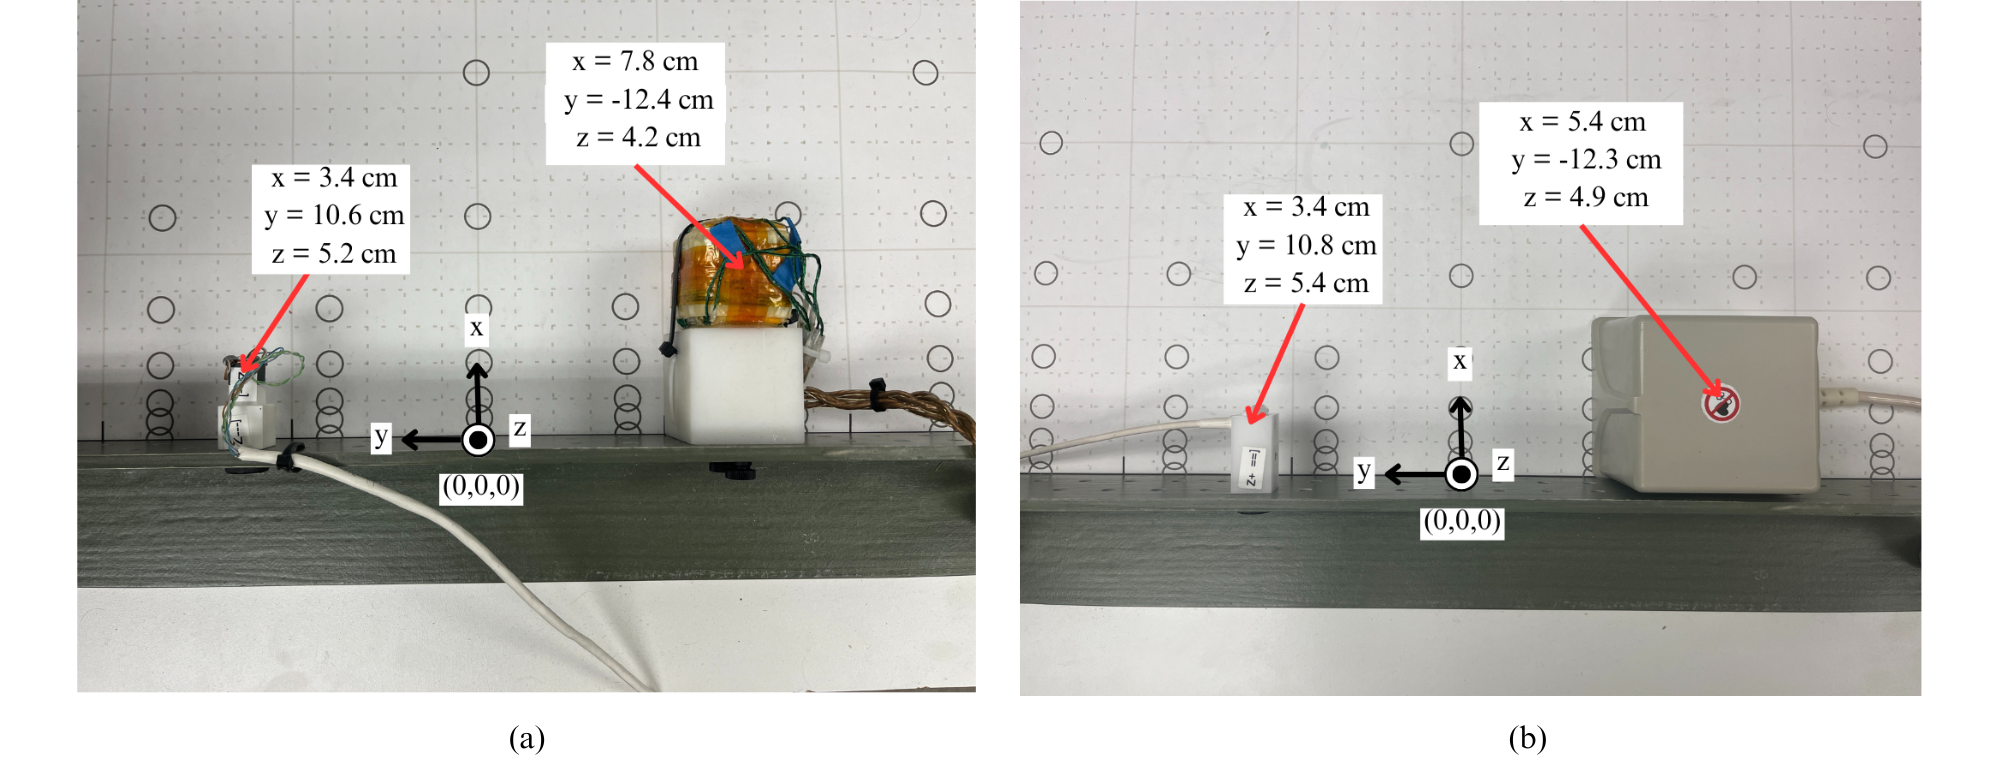
\includegraphics[width= 7in]{chaicS1.png}}
\caption{The configuration of source and sensor position of two trackers is relative to the global origin: (a) ILEMT and (b) 3D Guidance trakSTAR. The two components (source and sensor) are approximately 23 cm apart along the y-axis. There is a small discrepancy between two trackers due to the larger dimension of trakSTAR transmitter than ILEMT source. The global origin is located at the middle with three axes direction.}
\label{configuration}
\end{figure}

Two main coils of ILEMT were fixed in the workspace. The sensor was at (3.4, 10.6, 5.2) cm, while the source coil was at (7.8, -12.4, 4.2) cm from the global origin, as shown in Fig. \ref{configuration} (a).

LABVIEW was used for ILEMT data acquisition. The raw data was coupling matrices which we post-processed in MATLAB to generate the pose solutions. We converted the pose difference between the metal and no-metal conditions into 3-DOF translation and rotation vectors. The scalar translation and rotation errors we report are the magnitudes of these vectors.

3D Guidance trakSTAR is a pulsed DC tracker used in performance comparison of ILEMT. It provides 6 DOF tracking with three translational dimensions (x, y, z) and three rotational dimensions (azimuth, elevation, roll) relative to the transmitter. We placed its sensor and transmitter at approximately the same coordinates as the ILEMT coils. The sensor was at (3.4, 10.8 cm, 5.4 cm), while the transmitter was at (5.4, -12.3, 4.9) cm, as shown in Fig. \ref{configuration} (b).

We also collected data using LabVIEW at measurement rate of 80 Hz with the built-in toolbox of the 3D Guidance trakSTAR system. The raw data included three translational and three rotational components, matching the pose solution format of ILEMT, which allowed us to compute and compare errors across varying distances.

\section{Pulsed vs. Low AC fields across three shapes}
\label{supplement:pulse_Low}

\begin{figure}[!htbp]
\centerline{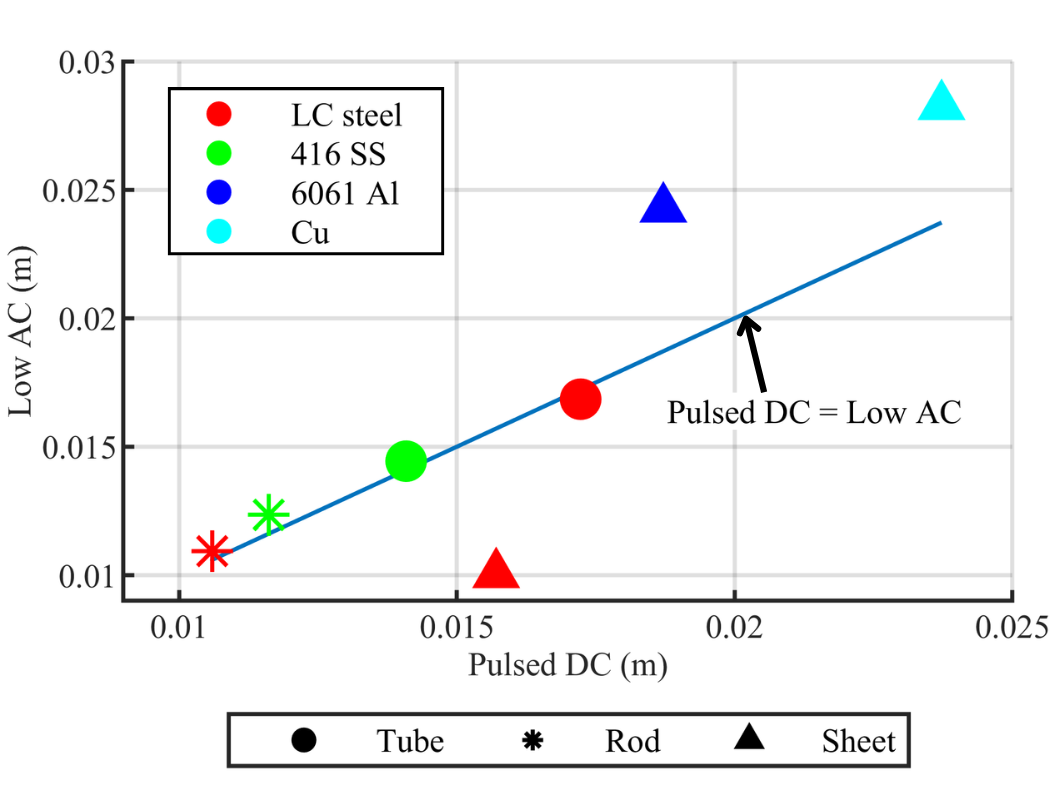
\includegraphics[width= 3.5in]{chaicS2.png}}
\caption{The scatter plot of translation error, comparing of pulse modulation and Low AC. The errors for the ferromagnetic rod and tube samples are almost identical across the modulations, and for the sheets the relative mismatch is still small.  Rods and tubes are placed at $x=10$ cm, and sheets are placed at $x=18$ cm to fit the markers within this plot.
(Modulations: Low AC and Pulse, Shapes: All, Positions: (10, 0) and (18, 0), Rotation: $0^\circ$)}
\label{3DGuidance_Low_compare}
\end{figure} 

In Fig. \ref{3DGuidance_Low_compare}, the scatter plot shows the variation of response when the metal shape changes. Only ferromagnetic materials are measurable by trakSTAR, but all sheet samples are detectable, even for non-ferromagnetic 6061 Al and Cu. The response of small samples, rod and tube, is on the unity line, which specifies the mostly identical response between Low AC and pulsed DC. The larger volume of metal deviates the response from the identical line. 

\section{Sheet Interference Mechanisms}
\label{supplement:sheet_interference}

Why does the sheet rotation have such a large effect, especially on the metal type and modulation interactions? Refer back to Fig. \ref{magnetic_field}, which visualizes the source magnetic field lines and metal orientation. The field lines which would pass through the metal location and also reach sensor will pass the metal roughly parallel to the $0^\circ$ rotation (primarily the $x$ field). In this orientation (Fig. \ref{sheet_0deg}) the field sees the small cross section of the metal edge, so relatively small eddy currents are induced. But some $y$ field lines which would otherwise \textit{not} reach the sensor see the broad face of the sheet, creating a very large eddy current loop. This eddy current reflects those source fields toward the sensor. 
 
Since the loop is very large, the inductance is also large, and it is this inductance that determines the eddy current strength, not the metal conductivity (as for high conductivity metals in the loop model, \S\ref{subsubsec:eddy_current_model}.) So the interference in Fig. \ref{sheet_0deg} is the same at High AC modulation for all non-ferromagnetic metals, even the low conductivity 304 SS.

To understand the effect of the ferromagnetic LC Steel we must consider how rotation affects its demagnetization. The parallel $x$ field sees high magnetization of the metal which will have some effect on the field at the sensor, but in the $0^\circ$ rotation this effect is apparently overpowered by the eddy current field reflection. The permeability effect on the $y$ field and its reflection is minimal because demagnetization is very high for this field. So LC Steel just behaves as a moderate conductivity metal. Despite its nominally higher permeability at Low AC, it shows \textit{reduced} interference, intermediate between the high conductivity and low conductivity non-ferromagnetic metals.

At the $90^\circ$ rotation (Fig. \ref{sheet_90deg}), the sheet eddy current does not reflect any source field toward the sensor, and the main effect for non-ferromagnetic metals is attenuating the $x$ source field. The frequency response follows the correlation with skin depth that we observed for rods and tubes, and as for tubes the low conductivity 304 SS nearly disappears at Low AC modulation and $90^\circ$ rotation. At this rotation the ferromagnetic LC Steel also shows the increase in interference at Low AC which was seen with rods and tubes, so permeability effects are once again significant.


\section{Power law fit of rod samples}
\label{supplement:rod_fitting}
\begin{figure}[!htbp]
\centerline{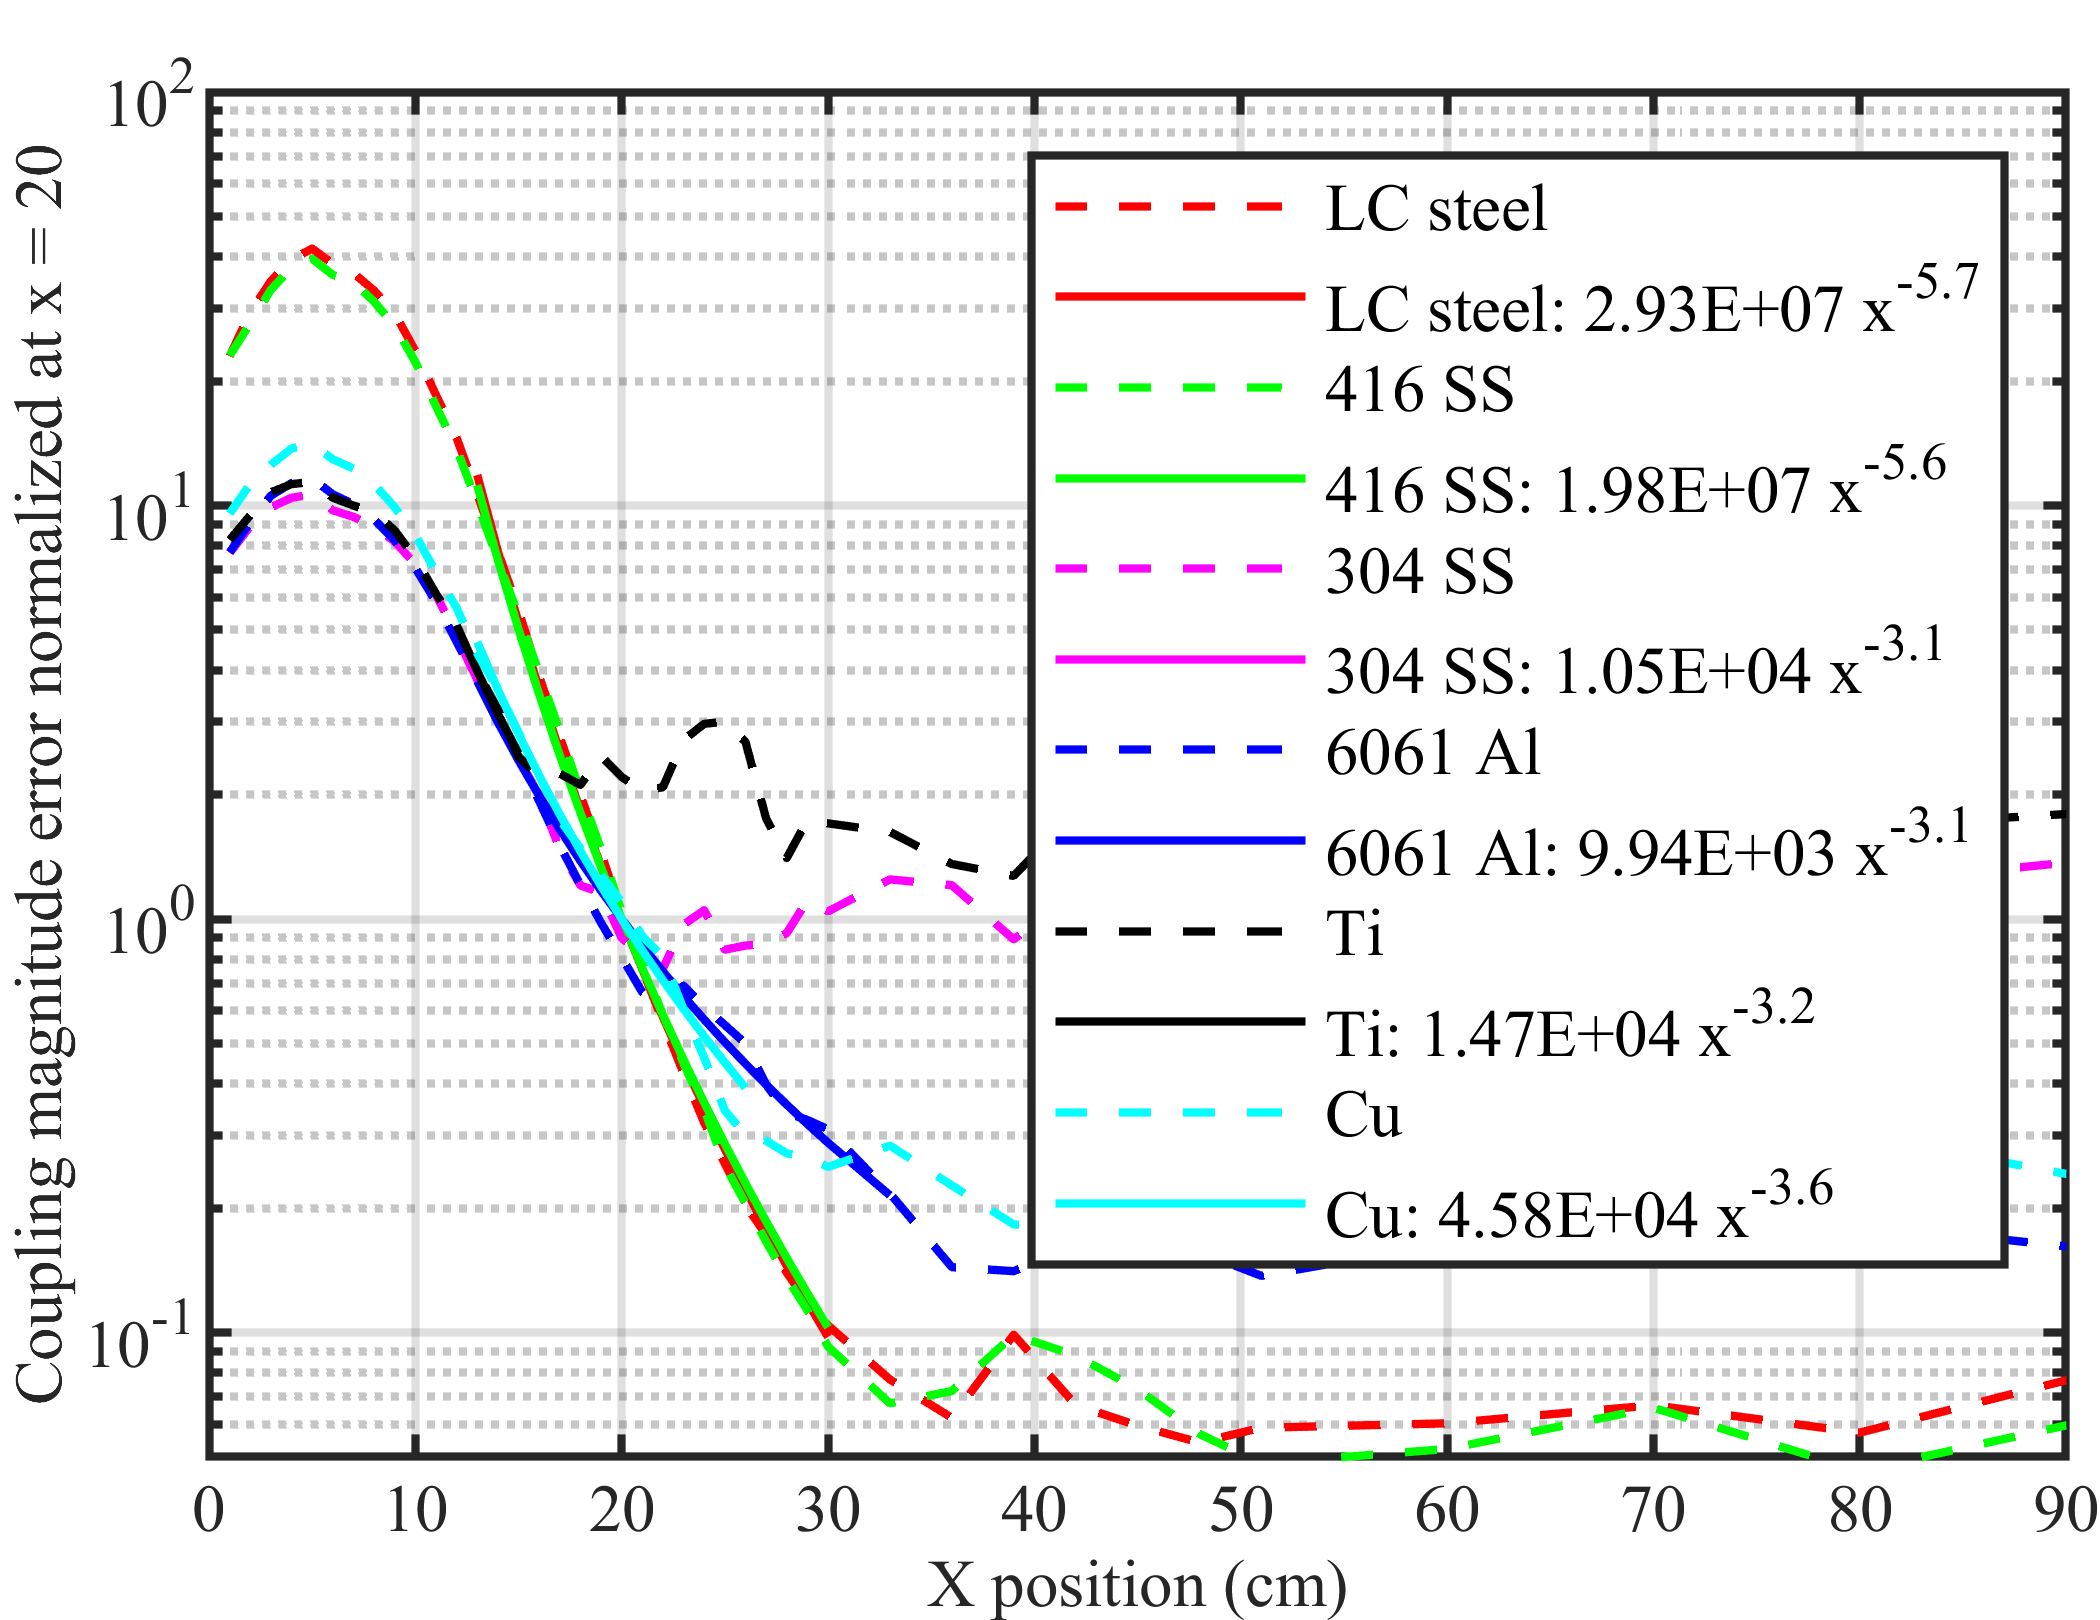
\includegraphics[width= 3.5in]{chaicS3.png}}
\caption{Power law fit of coupling error magnitude response to $x$ motion for rods. The data for each sample is normalized so that the curve fit passes through (20, 1). Two distinct responses are observed: ferromagnetic and non-ferromagnetic materials show similar patterns to their tube fitting. The exponent of non-ferromagnetic metals has lower magnitude than ferromagnetic metals, and also shows the least magnitude compared to tube samples. 
(Shapes: Rod, Modulation: High AC, Rotation $0^\circ$).}
\label{rod_fit}
\end{figure} 

Metal shapes and types influence the drop-off characteristics. Fig. \ref{rod_fit} shows that ferromagnetic rod samples exhibit an exponent close to -6, similar to ferromagnetic tube samples. Non-ferromagnetic rod samples display a less steep slope compared to their tube responses. These non-ferromagnetic rod samples also show the lowest magnitude among all power law fits.

\section{Power law fit of sheet samples}
\label{supplement:sheet_fitting}
\begin{figure}[!htbp]
\centerline{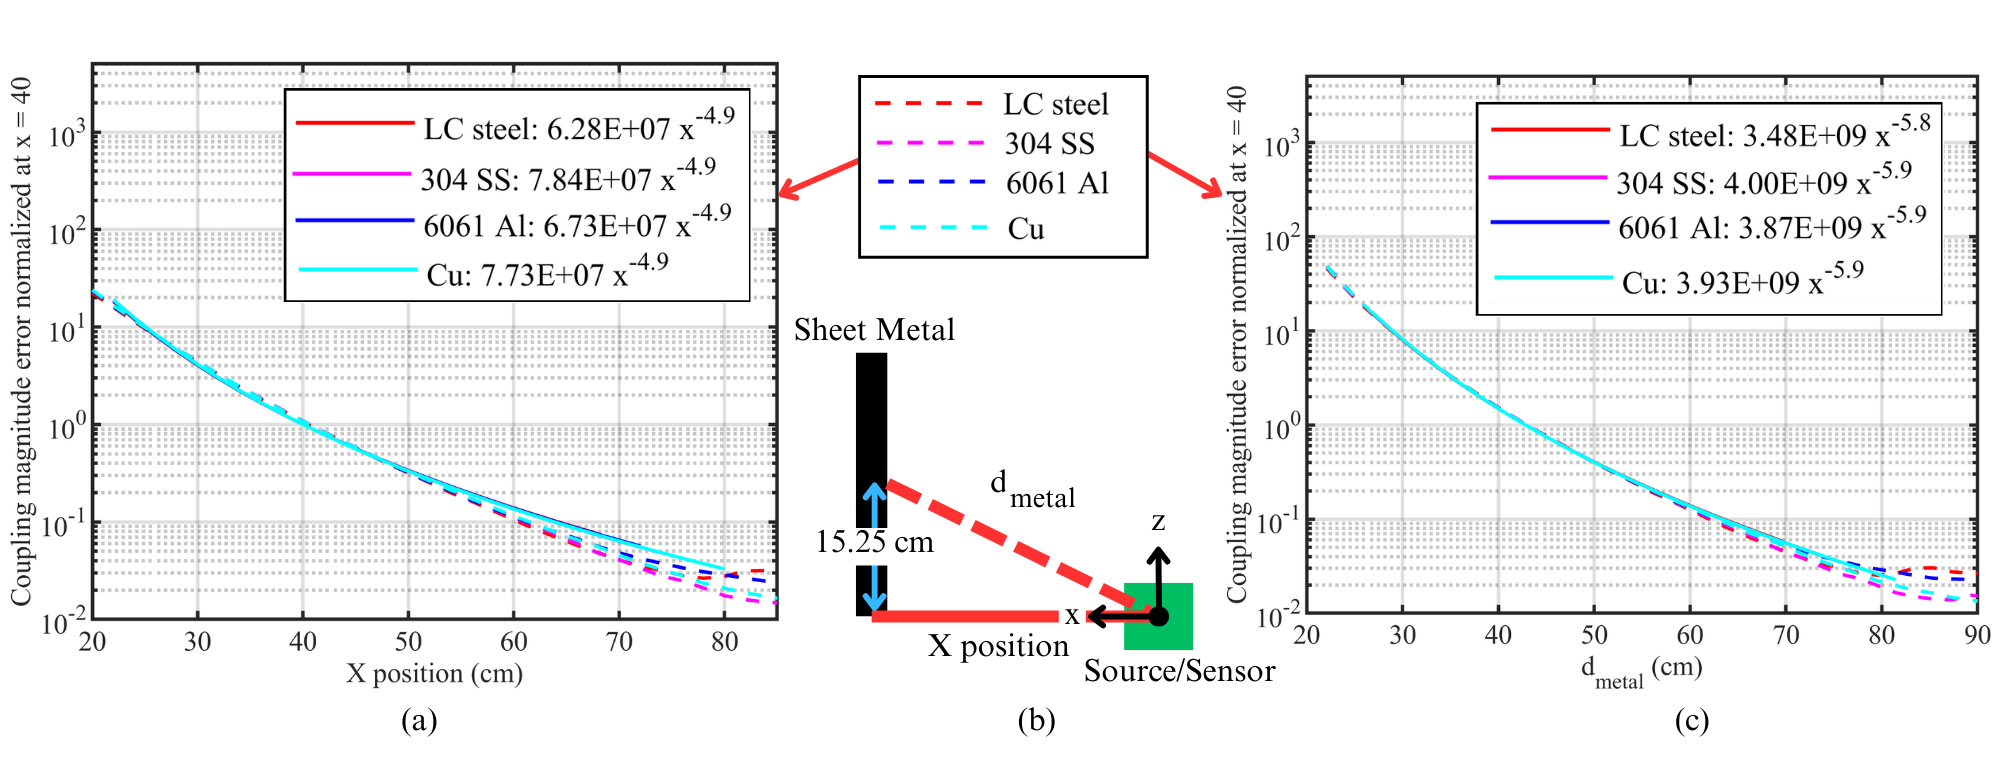
\includegraphics[width= 7in]{chaicS4.png}}
\caption{Power law fit of sheet samples normalized at x = 40 cm with high AC and 0-degree orientation: (a) relative to the x-coordinate, and (c) relative to the distance from the origin to the center of mass. (b) Geometry correction from the x-position to the actual distance to the center of mass. The results show an increase in the exponent magnitude, approaching -6 after the correction. (Shapes: Sheet, Modulation: High AC, Rotation $0^\circ$).}
\label{coupling_sheet_fit}
\end{figure} 

Fig.\ref{coupling_sheet_fit} shows the power law fits for sheet metal. After a geometric correction for the height of the metal center above the source-sensor plane we found an excellent fit for $d_{\text{metal}}^{-5.9}$. Rotating the sheet to $90^\circ$ gives similar behavior (not shown.)

\section{Nixon model agreement}
\label{supplement:Nixon_ratio}
As shown in Fig. \ref{Nixon_ratio}, the ratio of the measured error to $d_{se}^{-3}d_{so}^{-3}$ does not remain constant, so the fit to the Nixon model\cite{nixon_effects_1998} is poor until $x>25$\,cm, at which point there is very little error in any case. For sheets, after the geometric correction above (\S\ref{supplement:sheet_fitting}), agreement with the Nixon model is good.

\begin{figure}[!htbp]
\centerline{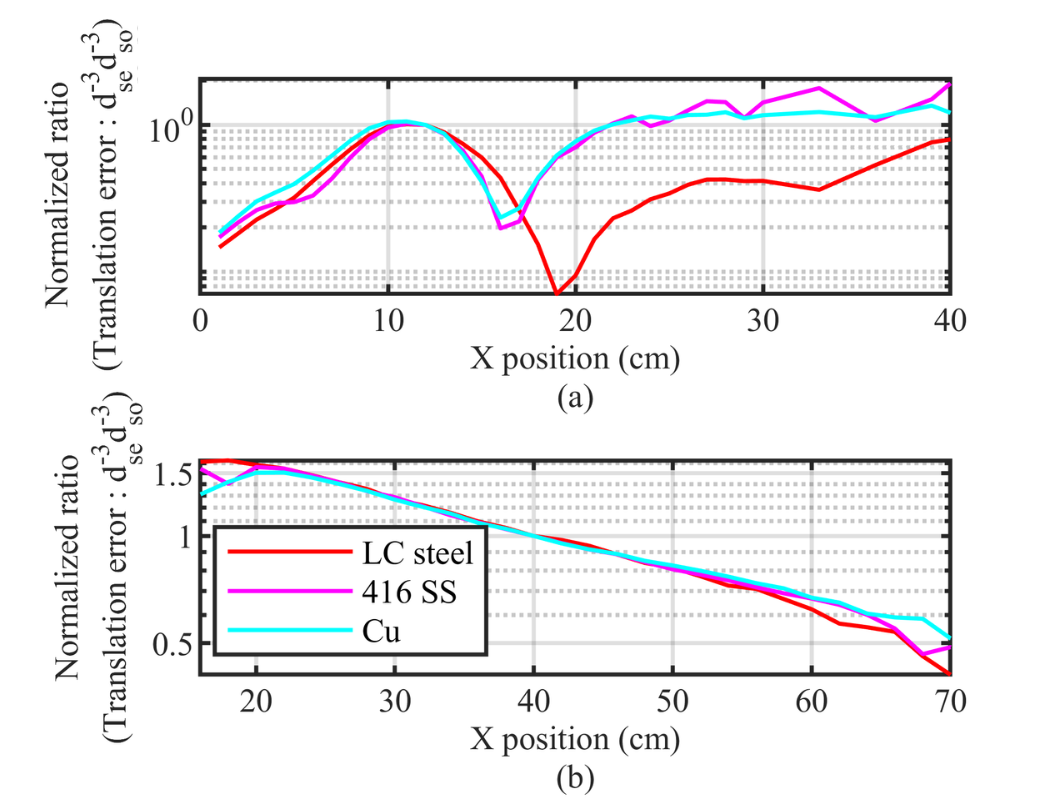
\includegraphics[width=3.5in]{chaicS5.png}}
\caption{Ratio of translation error to ${d_{se}^{-3} d_{so}^{-3}}$ with (a) normalized at x = 12 cm for tube LC steel and (b) normalized at x = 40 cm for sheet metal.}
\label{Nixon_ratio}
\end{figure} 

\end{document}